\documentclass[conference]{IEEEtran}
\IEEEoverridecommandlockouts
% The preceding line is only needed to identify funding in the first footnote. If that is unneeded, please comment it out.
\usepackage{cite}
\usepackage{amsmath,amssymb,amsfonts}
\usepackage{mathtools}
\usepackage{algorithmic}
\usepackage{graphicx}
\usepackage{textcomp}
\usepackage{xcolor}
\usepackage{gensymb}
\usepackage{url}
\def\BibTeX{{\rm B\kern-.05em{\sc i\kern-.025em b}\kern-.08em
    T\kern-.1667em\lower.7ex\hbox{E}\kern-.125emX}}
\begin{document}

\title{Feasibility of Gradient-Based Optimizations in General Relativity\\
% {\footnotesize  \textcolor{white}{Some white words to space things out}}
% \thanks{Identify applicable funding agency here. If none, delete this.}
}

\author{\IEEEauthorblockN{Qijie (Jay) Feng}
\IEEEauthorblockA{\textit{} jfeng8035@gmail.com}
% \and
% \IEEEauthorblockN{2\textsuperscript{nd} Given Name Surname}
% \IEEEauthorblockA{\textit{dept. name of organization (of Aff.)} \\
% \textit{name of organization (of Aff.)}\\
% City, Country \\
% email address or ORCID}
% \and
% \IEEEauthorblockN{3\textsuperscript{rd} Given Name Surname}
% \IEEEauthorblockA{\textit{dept. name of organization (of Aff.)} \\
% \textit{name of organization (of Aff.)}\\
% City, Country \\
% email address or ORCID}
% \and
% \IEEEauthorblockN{4\textsuperscript{th} Given Name Surname}
% \IEEEauthorblockA{\textit{dept. name of organization (of Aff.)} \\
% \textit{name of organization (of Aff.)}\\
% City, Country \\
% email address or ORCID}
% \and
% \IEEEauthorblockN{5\textsuperscript{th} Given Name Surname}
% \IEEEauthorblockA{\textit{dept. name of organization (of Aff.)} \\
% \textit{name of organization (of Aff.)}\\
% City, Country \\
% email address or ORCID}
% \and
% \IEEEauthorblockN{6\textsuperscript{th} Given Name Surname}
% \IEEEauthorblockA{\textit{dept. name of organization (of Aff.)} \\
% \textit{name of organization (of Aff.)}\\
% City, Country \\
% email address or ORCID}
}

\maketitle

\begin{abstract}
Recent advances in the field of machine learning have successfully 
employed gradient-optimized neural network models in solving real-world 
physical problems regarding dynamical systems. However, most 
approaches heavily rely on the use of surrogate models which 
approximates the actual physical laws. In this work, we investigate 
the feasibility of adopting gradient-based optimization directly 
to numerical General Relativity simulations, driven by exact 
physical principles, for solving correct initial conditions. 
A toy problem is proposed to evaluate the performance of optimization 
methods. We compare two approaches for gradient-based optimization $-$ 
direct differentiation over the ODE solver and the adjoint sensitivity method, 
with performance assessed on both static and evolving spacetime metrics. 
Experiments demonstrate that the adjoint sensitivity method 
achieves stable convergence, while direct differentiation over the 
solver suffers from numerical instabilities and chaotic behavior near 
the optimum. Our results indicate that gradient-based optimization 
can indeed be applied directly to the context of General Relativity; 
with careful choice of numerical methods, gradient-based optimization 
can potentially be powerful tools in analyzing a large number 
of dynamical systems.
\end{abstract}


\section{Introduction}
Gradient-based optimization has achieved great success in 
the field of machine learning, allowing the development of 
numerous modern statistical algorithms that automatically 
“learns” the underlying distributions of complex data. neural 
network-based models, in particular, has found applications 
in various of fields outside of mathematics and computer 
science (e.g., medicine, physics, economics, etc.) Recently, 
many efforts are made to utilize the strong representativity of 
neural network-based methods for applications in modeling 
dynamical systems. For example, Physics-Informed Neural Networks 
(PINN) \cite{PINN} has been proven powerful in modeling 
astronomical shock waves in a 2023 paper \cite{PINNapp}. 
FourCastNet \cite{FourCastNet}, a model developed by Nvidia, 
achieved short to medium-range global weather prediction up to 
a resolution of $0.25^\circ$, using neural networks that learns 
the features of functions from the Fourier domain \cite{FourOp}. 

These successes shows also the remarkable effectiveness of 
optimization $-$ the fundamental tool enabling machine learning 
models to “learn” $-$ in handling complex physical systems driven 
by ordinary or partial differential equations. However, most 
existing applications rely on a surrogate model, such as a neural 
network, that approximates the underlying physics. Far fewer 
attempts are made to apply optimization directly to the parameters 
of a dynamical system governed strictly by physical laws. 

Particularly, we noticed a gap in employing optimization methods 
to parameters of General Relativity, and having its dynamical 
evolution controlled only by the physical and geometrical laws 
of the Einstein equations, not that of a learned representation. 
This leads to our research question: 
\begin{itemize}
    \item Can gradient-based optimization methods $-$ proven robust in machine learning $-$ be feasibly applied to General Relativity's dynamical systems, especially in determining the structure of spacetime geometries?
\end{itemize}
	
To answer it, this paper first proposes a toy problem, 
involving conditions that determine the geometrical structure of 
spacetime through General Relativity and an implicit way to 
measure such structures. Then the performance of gradient-based 
optimization on this toy problem is evaluated, as well as 
the numerical stability of its convergence to the solutions. 

This paper assumes an audience with only background in linear algebra 
and multivariable calculus. Thus, the crucial mathematical tools for 
constructing General Relativity spacetime will be briefly introduced 
and derived using language of linear algebra and multivariable calculus 
in the following \textit{Preliminary} section.


\section{Preliminaries}

\subsection{Describing Curved Spaces}

An easy way of observing the intrinsic curvature of a space is to see how
the space's measure of length or inner product deviates from that
of Euclidean space. For example, a straight line on a Mercator-projected 
map of the Earth is often not straight on the land, nor is it the 
shortest path connecting the two endpoints. On the other hand, the shortest 
route connecting two locations on Earth, the great circle, is often not a 
straight line on the map, unless it is a part of the equator or a meridian. 
To analytically understand the curvature of space, we need a way to mathematically 
interpretate the space's deviation from the Euclidean space, and thus is the notion 
of metric introduced.

An intuition can be drawn from the law of cosine:
\[
c^2 = a^2 + b^2 - 2ab\cos(\theta)
\]
where one sees that when the basis vectors of $\mathbb{R}^2$ are not orthonormal 
(i.e., $e_i \cdot e_j = 0$ if $i \neq  j$, and 1 otherwise), the length of some vector, 
say $-e_1 + e_0$ 
in the space may take the form $||v|| = \alpha e_0 \cdot e_0 + \beta e_1 \cdot e_1 + \gamma e_0 \cdot e_1$,
for $\alpha,\beta,\gamma \in \mathbb{R}$ Hence, we may define the metric 
of a $\mathbb{R}^2$ space as associated to the length of an infinitesimal vector:
\[
ds^2 = \alpha dx^2 + \beta dy^2 + \gamma dxdy,
\]
where $\alpha, \beta, \gamma$, being scalars, measure the amount of variation from the Rule of Pythagoras. 
It is worth to realize that the space the matric describe can have far 
more complicated geometrical structures, where the measure of length varies 
at every point in the space. Thus, $\alpha, \beta,$ and $\gamma$ are really 
scalar fields which take in a position $\mathbf{x}$: $\alpha(\mathbf{x}), \beta(\mathbf{x}),
\gamma(\mathbf{x})$, but for conciseness, the arguement $(\mathbf{x})$ is usually omitted.
The form above for a metric, as an equation describing how infinitesimal length $ds$ shall be calculated, may seem clear enough, but problems soon arise when the number 
of dimensions increase. For example, a 3-dimensional metric requires 6 irreducible terms, 
whereas a 4-dimensional one requires 10. Thus, to avoid this cumbersomeness,
a metric is commonly written as a matrix. For example, in the the case of $\mathbb{R}^2$
\[
M =
\begin{bmatrix}
\alpha & \gamma \\
\gamma & \beta
\end{bmatrix},
\]
where $ds^2$ becomes
\[
ds^2 = \mathbf{dx}^\top M \, \mathbf{dx}
\quad \text{for } \mathbf{dx} = \begin{bmatrix} dx \\ dy \end{bmatrix}
\tag{1}
\]

Next, we examine some properties of the metric. First consider a coordinate 
change $x \rightarrow x' = f(x)$. The differentials in the new coordinate system becomes
$\mathbf{dx}' = J_{x \rightarrow x'} \mathbf{dx}$, where $J_{x \rightarrow x'}$ denotes the Jacobian matrix for the coordinate 
transformation from $x$ to $x'$. Substitute this into eq. (1) and noting that the length 
of a vector shall not change under coordinate changes (think about doing integration 
and transforming to polar/spherical coordinate: the result of the intergation 
shall not vary no matter what coordinate you choose). This yields:
\begin{align*}
ds'^2 &= \mathbf{dx}'^\top M' \mathbf{dx} \\
&= (J_{x \rightarrow x'} \mathbf{dx} )^\top M' (J_{x \rightarrow x'} \mathbf{dx} ) \\
&= \mathbf{dx}^\top (J_{x \rightarrow x'}^\top M' J_{x \rightarrow x'}) \mathbf{dx} = ds^2
\end{align*}
For the last line to hold, $M$ must transform by:
\[
M' = {J_{x \rightarrow x'}^{-1}}^\top M J_{x \rightarrow x'}^{-1}.
\]
Denoting the component at the $\alpha$-th row, $\beta$-th column of $M$ as $g_{\alpha\beta}$, and 
realizing that the component at the $i$-th row, $j$-th column of the inverse Jacobian 
can be written in terms of the partial derivative of the coordinate functions 
$\partial x^i / \partial x^{\prime j}$ (superscripts here represent index, not exponents), an explicit formula can be written for $g'_{\mu\nu}$, 
the components of $M'$:
\[
g'_{\mu\nu} = \sum_{\beta=1}^n 
\sum_{\alpha=1}^n g_{\alpha\beta} \frac{\partial x^\alpha}{\partial x'^\mu} 
\frac{\partial x^\beta}{\partial x'^\nu},
\tag{2}
\]
where $n$ is the number of dimensions the space which $M'$ describes has. A deriviation of 
eq. (2) is provided in Appendix 1.

Looking at the effect of applying a metric to a vector reveals its nature 
of being a tensor $-$ a multilinear mapping. Let us start by considering the essence of vectors. Suppose we have a vector $\mathbf{v}$, representing 
a relative position in the space where length is defined by the metric $M$. 
Such a vector's components are “contravariant”, meaning they change in reverse to 
the coordinate change. Intuititively, given that the length of a vector needs 
to be perserved, the post-coordinate change components of $\mathbf{v}$ have to, for example, 
expand if the transformation has shrunk the coordinate grid. 

For a formal definition of a vector, we shall observe that vector arises from changes 
(e.g., changes in position, velocity, etc.), so it is reasonable to define 
their components as the change of coordinate value with respect to some parameter $\lambda$:
\[
v^i = \frac{\partial x^i}{\partial \lambda} \quad\quad
v'^i = \frac{\partial x'^i}{\partial \lambda}
\]
where $v^i$ and $v'^i$ represents the $i$-th value of vector $\mathbf{v}$ and $\mathbf{v'}$
(the vector after coordinate transformation), respectively; $x^i$ is the coordinate value along 
the $i$-th direction. Applying the chain rule on $v'^i$ yields:
\[
{v'}^i=\frac{\partial{x'}^i}{\partial\lambda}
=\sum_{j}{\frac{\partial{x'}^i}{{\partial x}^j}\frac{\partial x^j}{\partial\lambda}}
=\sum_{j}{\frac{\partial{x'}^i}{{\partial x}^j}v^j}
\tag{3}
\]
This is the contravariant transformation rule for vectors. We may put 
our focus on the scaling factor $\partial{x'}^i/\partial x^j$, as this 
would help us determine whether or not a set of vector components transforms 
contravariantly. With this in mind, we now look at the properties of $M \mathbf{v}$ 
and the transformed product $M' \mathbf{v}'$. Let $v_\mu$ and $v'_\mu$ be the $\mu$-th 
component of $M \mathbf{v}$ and $M' \mathbf{v}'$, respectively (subscript is used here 
to conform to the convention of tensor calculus, which will be introduced later). Then,
\[
v'_\mu = \sum_{\nu}{{g'}_{\mu\nu}{v'}^\nu}
\]
This is simply writing the matrix-vector product out as a summation. Now substitute in 
eq. (2):
\[
v'_\mu = \sum_{\nu}
\left(\sum_{\beta} 
\sum_{\alpha} g_{\alpha\beta} \frac{\partial x^\alpha}{\partial x'^\mu} 
\frac{\partial x^\beta}{\partial x'^\nu}\right)
v'^\nu,
\]
and the contravariant transformation rule for $v'^\nu$:
\begin{align*}
v'_\mu &= \sum_{\nu}
\left(\sum_{\beta} 
\sum_{\alpha} g_{\alpha\beta} \frac{\partial x^\alpha}{\partial x'^\mu} 
\frac{\partial x^\beta}{\partial x'^\nu}\right)
\sum_{j}{\frac{\partial{x'}^\nu}{{\partial x}^j}v^j} \\
&=
\sum_{\nu} \sum_{\beta} 
\sum_{\alpha} \sum_{j} \frac{\partial x^\alpha}{\partial x'^\mu} 
\frac{\partial x^\beta}{\partial x'^\nu}
\frac{\partial{x'}^\nu}{{\partial x}^j}
g_{\alpha\beta} v^j
\end{align*}
The summation 
$\sum_{\nu}\frac{\partial x^\mu}{{\partial x'}^\nu}\frac{\partial{x'}^\nu}{{\partial x}^j}$
is equivalent to the matrix multiplication between a Jacobian matrix and its inverse, 
hence acts like the identity matrix when indexed by $\beta$ and $j$. We can safely 
omit the summation as it imposes only an identity transformation to $g_{\alpha\beta} v^j$.
However, since we are treating the product between the identity matrix and 
$g_{\alpha\beta} v^j$ as a whole, the index $\beta$ we sum over becomes $j$, as if 
we are summing over the column index of 
$\frac{\partial x^\beta}{{\partial x'}^\nu}\frac{\partial{x'}^\nu}{{\partial x}^j}$:
\begin{align*}
v'_\mu &= 
\sum_{\alpha} \sum_{j} \frac{\partial x^\alpha}{\partial x'^\mu} 
g_{\alpha j} v^j \\
&=
\sum_{\alpha} \frac{\partial x^\alpha}{\partial x'^\mu} 
\sum_{j} g_{\alpha j} v^j
\end{align*}
This reveals a different transformation factor $-$ the components of the inverse Jacobian 
$J_{x \rightarrow x'}^{-1}$ 
We call any quantities that transforms according to this rule covariant. 
Covariant vectors, or ``convectors" has the property of changing along coordinate changes. 
This change cancels with that of contravariant vectors in eq (3), resulting in an 
invariant quantity when being multiplied $-$ the squared length of vector $\mathbf{v}$: 
$||\mathbf{v}||^2 = \mathbf{v}^\top M \mathbf{v}$

Looking at this quadratic form, one may sense some unnaturalness $-$ the fact 
that vector dot products $\mathbf{v}^{\mathsf{T}} \mathbf{u}$ has lost its 
geometric meaning as in the Euclidean space, but becomes only a notation of 
summation. To compensate with this, a more useful and intuitive 
definition is established, that convectors are actually functionals: mappings 
from a vector space to $\mathbb{R}$. Thus, the invariant length of vectors 
turns into the result of a convector “acting” upon a contravariant one: 
$||\mathbf{v}||^2 = \mathbf{v}^{\mathsf{T}} M \mathbf{v} = 
\mathbf{v}_{\text{covect}}(\mathbf{v}_{\text{contravect}})$ Furthermore, the 
functional $\mathbf{v}_{\text{covect}}$ shall be linear (i.e., 
$\mathbf{v}_{\text{covect}}(\mathbf{u}+\mathbf{w})=\mathbf{v}_{\text{covect}}(\mathbf{u})+
\mathbf{v}_{\text{covect}}(\mathbf{w})$; $\mathbf{v}_{\text{covect}}(\lambda \mathbf{u})=\lambda 
\mathbf{v}_{\text{covect}}(\mathbf{u})$ for vectors $\mathbf{u}, \mathbf{w}$ and scalar $\lambda$), 
as to conform to the linearity of summation. This allows us to also 
define the essence of metrics as being tensors: a multilinear mapping from either
\begin{enumerate}
    \item the product of two vector space to $\mathbb{R}$, or
    \item a vector space $V$ to a space of linear functionals $V^*$ 
    in which $\omega: V \rightarrow \mathbb{R} \quad \forall \omega \in V^*$.
\end{enumerate}
Of course, tensors in general can take many other forms of mapping 
(e.g., $V^* \times V \rightarrow \mathbb{R}$), but defining a metric as a tensor of the above 
mapping certainly provides a more natural perspective for understanding 
such mathematical objects.

For the rest of this paper, two conventions will be used: tensor calculus 
and Einstein summation notation. With tensor calculus, contravariant vector 
components are denoted with upper indices: $v^i$, and covariant components are 
denoted with lower indices: $v_i$; with Einstein summation notation, we sum over 
repeated indices in a term, and an ease in formulation follows:
\[
\mathbf{v}_{\text{covect}}\left(\mathbf{v}_{\text{contravect}}\right)=
v^i v_i \coloneqq \sum_{i}{v^iv_i}
\]
It appears that, formally, the indices cancel with each other. Similarly, 
for between metric tensors and vectors:
\[
v_\mu=g_{\mu\nu}v^\nu \coloneq \sum_{\nu} g_{\mu\nu}v^\nu
\]
This method, known as tensor contraction, help us efficiently deal with 
coordinate changes and contravariant-covariant component conversions in which 
nested summations can be omitted. 

Noticing that the metric tensor has the ability of lowering the index of a 
vector component (i.e., convert it from contravariant to covariant), while 
itself also acts like a matrix. The reader may question whether the inverse 
of the metric matrix has the ability to raise indices. Indeed, the inverse metric, 
with components denoted $g^{\mu\nu}$ maps from a space of convectors $V^*$ to that of 
corresponding contravariant vectors $V$:
\[
v^\mu=g^{\mu\nu}v_\nu \coloneq \sum_{\nu} g^{\mu\nu}v_\nu
\]
A proof easily follows from the workflow in Appendix 1, by noting that 
$M'^{-1} = J_{x \rightarrow x'}^T M^{-1} J_{x \rightarrow x'}$.

\subsection{Path of Light and Some Geometrical Tools}
It can be shown (see Appendix 2) that the curve $X^\lambda$ describing trajectory of 
light in the coordinate system $x^\mu$
follows the differential equation
\[
\frac{\partial^2 X^\lambda}{\partial \sigma^2}
 = -\frac{1}{2} g^{\lambda\alpha} \left( \frac{\partial g_{\nu\alpha}}{\partial x^\mu}
+\frac{\partial g_{\alpha\mu}}{\partial x^\nu}
-\frac{\partial g_{\mu\nu}}{\partial x^\alpha}\right)
\frac{\partial X^\mu}{\partial \sigma}
\frac{\partial X^\nu}{\partial \sigma},
\tag{4}
\]
with parameterization $X^\lambda(\sigma)$. For light, this is known as the null 
geodesic equation. It turns out for no matter what quantities
we choose as the parameter, the differential equation would always produce the 
correct path of light when initial position and direction is specified. However, if 
we want the derivative $\partial X^\lambda /\partial \sigma$ to be physically 
meaningful, then there is limited options of how we can parameterize.

Comparing Minkowski spacetime with curved ones, one shall see 
that the flatness of the former leads to the vanishing of the metric tensor's derivative 
with respectively to coordinate directions, thus acceleration
$\partial^2X^\lambda / \partial\sigma^2 = 0$. The reader hence may recognize the 
significance of the factor 
$\frac{1}{2} g^{\lambda\alpha} \left( \partial g_{\nu\alpha} / \partial x^\mu
+\partial g_{\alpha\mu} / \partial x^\nu
-\partial g_{\mu\nu} / \partial x^\alpha\right)$ as somewhat imposing a gravitational 
force on light which deflects its path. Surprisingly, the factor acts more like 
countering any potential forces that light could be exerted with and allows light 
to travel naturally along the curvature of spacetime. We shall see that this factor 
emerges as a more fundamental element of curved space and enables us to define a 
generalized version of derivative along coordinate directions outside the Euclidean space. 

\begin{figure*}[htbp]
\centering
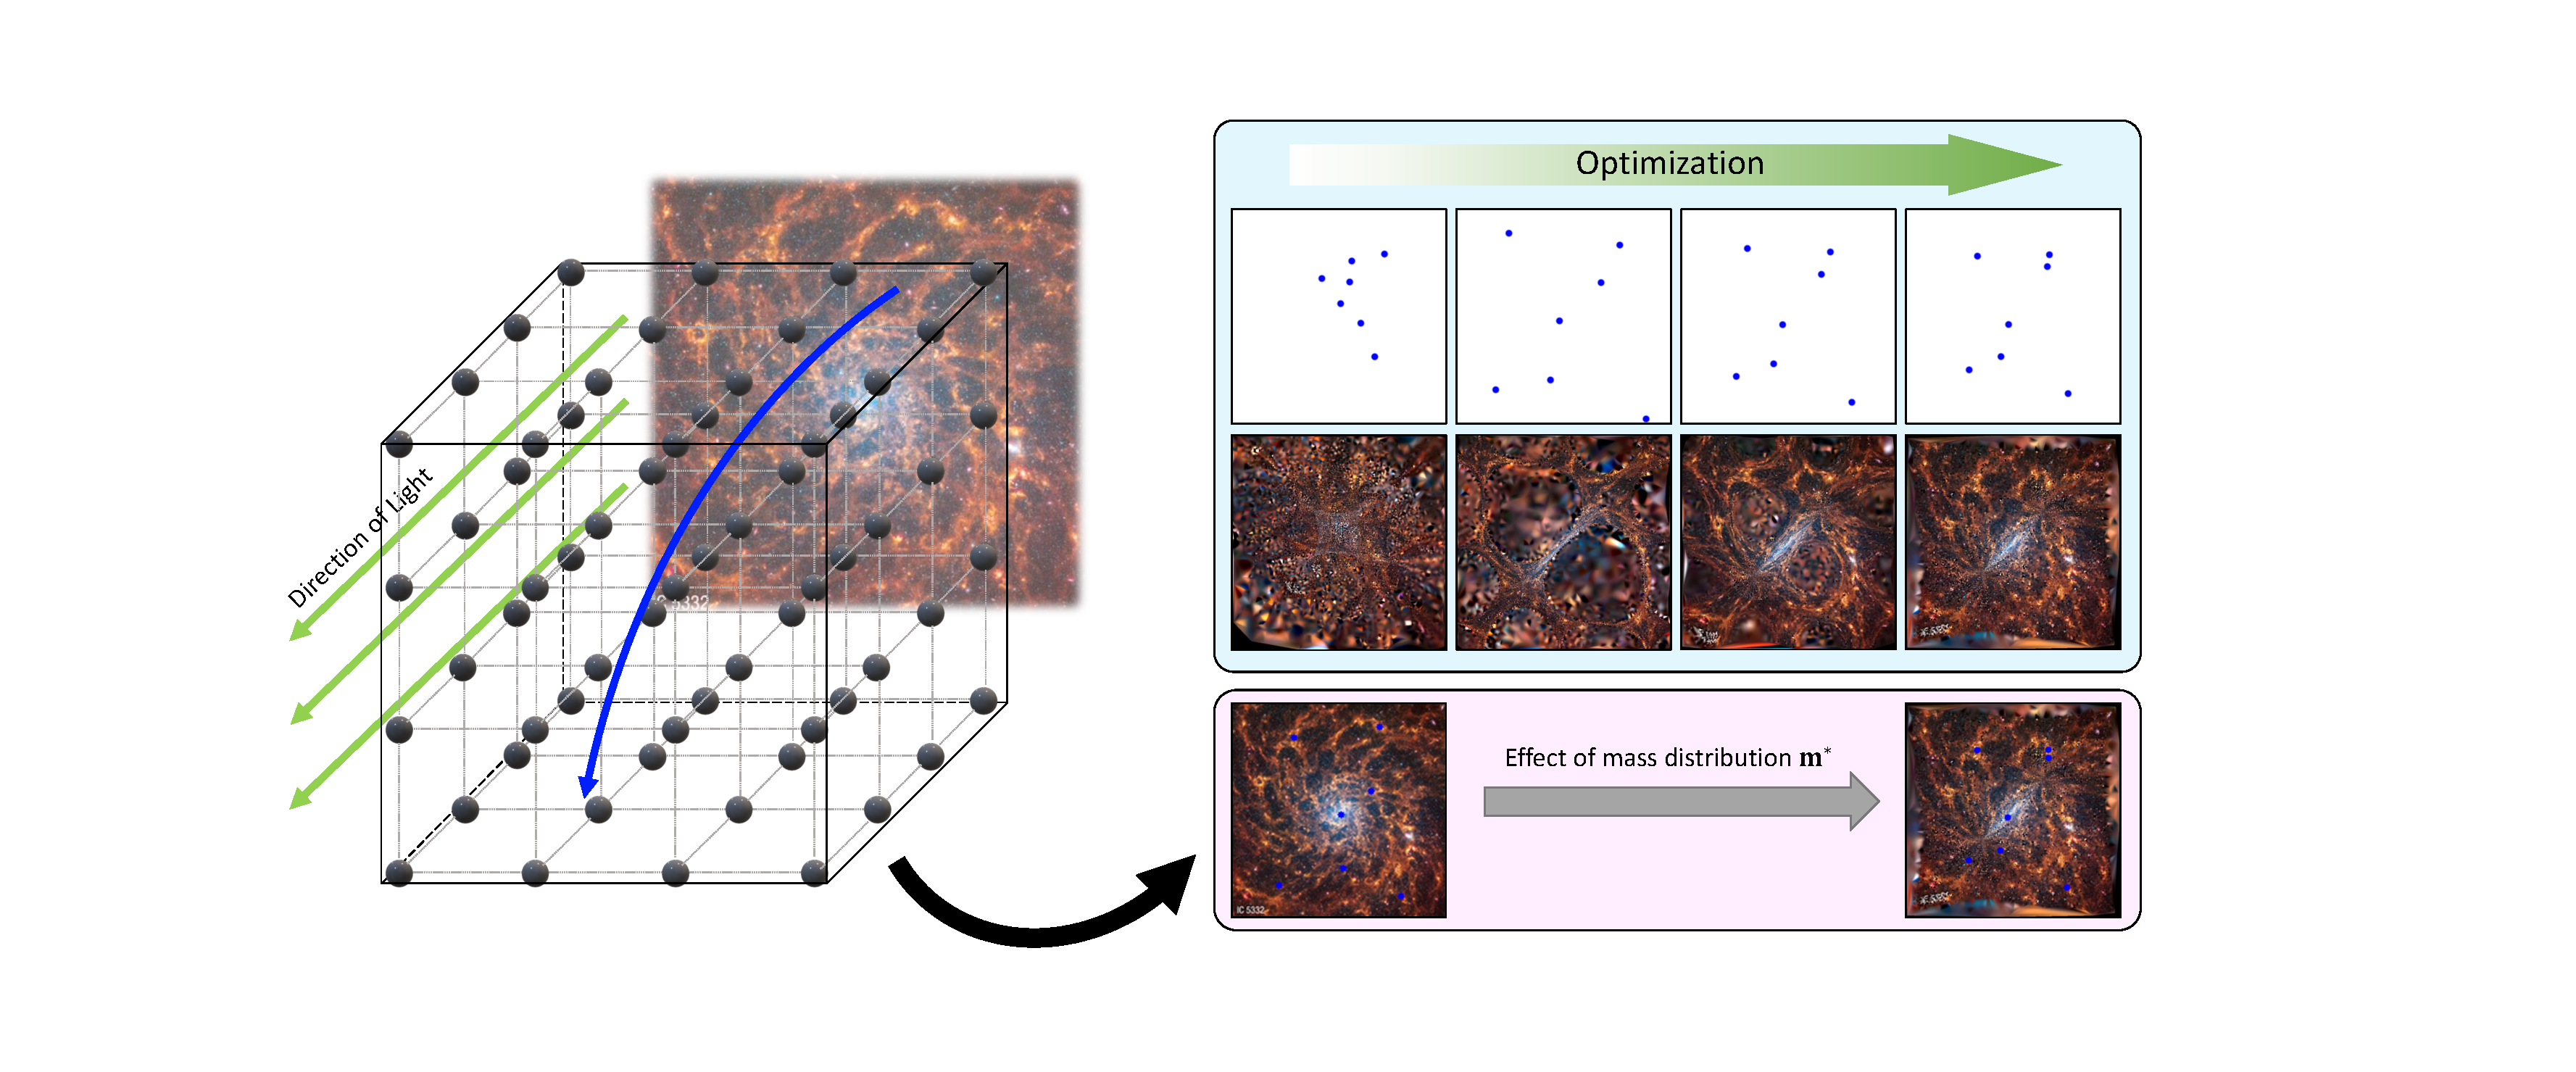
\includegraphics[width=\textwidth]{Fig1.pdf}
\caption{An illustration of the proposed toy problem for evaluating 
optimization performances. On the left is a visualization of the 
“blackhole grid” discretization of a mass distribution. 
This approach effectively approximates the spacetime containing the mass distribution
as a vacuum solution of Einstein 
equations. Light traveling through this region is deflected due to 
the curvature of the space. The pink panel shows how the induced 
curvature from mass distribution $\mathbf{m}^*$ distorts the image 
of a galaxy sitting behind the blackhole region. Blue dots indicate 
“structural landmarks” $\mathbf{y_0}_i$, which alters location to 
$\mathbf{y}_i$ as the trajectories of their light are curved. 
The blue panel demonstrates the optimization process, in which 
$\mathbf{m}$ is optimized via gradient-based methods so that the 
result of the solved propagations $\mathcal{S}(\mathbf{y_0}_i, \mathbf{m})$ 
matches with the observed $\mathbf{y}_i$. One can see that as 
optimization progresses, dots in blue panel get closer to locations 
marked in the right image of the pink panel. The second row in the blue 
panel demonstrates how the mass distribution $\mathbf{m}$ distorts the 
entire background throughout the course of optimization. }
\label{fig}
\end{figure*}

Consider a parallel transport, where a vector $\xi$ in coordinate system $x^\mu$ is transported 
along a direction on a curved surface such that for 
every infinitesimal interval which $\xi$ is transported along, 
the starting orientation and ending orientation of $\xi$ is 
parallel. In Euclidean space, this corresponds to the 
directional derivative of each component of $\xi$ being zero 
along the direction of transportation. It can be shown \cite{SemiR} 
that a generalized version of directional 
derivative $-$ the covariant derivative $-$ can be used to 
constrain the behavior of vector $\xi$ in curved spaces:
\begin{align*}
\nabla_\nu \xi^\mu :=& \frac{\partial \xi^\mu}{\partial x^\nu} + \frac{1}{2} 
g^{\mu k}\left(\frac{\partial g_{\nu k}}{\partial x^\lambda} + 
\frac{\partial g_{k \lambda}}{\partial x^\nu} - 
\frac{\partial g_{\lambda\nu}}{\partial x^k}\right) \xi^\lambda   \tag{5} \\
=& 0
\end{align*}
In spaces of no coordinate variation, that is, constant 
metric everywhere, the covariant derivative degenerates 
to directional derivatives along the coordinate 
directions, as described by the first term: $\nabla_\nu \xi^\mu=(\partial/\partial x^{\nu}) \xi^\mu$. 
When spatial curvature comes to play, however, 
the second term no longer stays zero, and acts 
like a correction term for directional derivatives 
that encodes the geometry of the space. One should recognize 
the familiar pattern, that the scaling factor 
in the second term is identical to the one 
we see in geodesic equation. Due to its significance and 
repeated occurrence of this factor in numerous aspects of 
differential geometry, and furthermore, 
the tensor-like property (index contraction works well in 
both the geodesic equation and covariant derivative), 
the factor is often denoted in a more concise manner, known as the 
Christoffel symbols:
\[
\Gamma_{\nu\lambda}^\mu := \frac{1}{2} 
g^{\mu k}\left(\frac{\partial g_{\lambda k}}{\partial x^\nu} + 
\frac{\partial g_{\nu k}}{\partial x^\lambda} - 
\frac{\partial g_{\nu\lambda}}{\partial x^k}\right)
\]
Both the covariant derivative and the Christoffel symbols are 
powerful tools we can use to formulate motions in curved spaces, and even 
evolutions of the spaces themselves, as we shall see from the \textit{Methodology} 
section below.




\section{Methodology}
This paper aims to investigate the feasibility of performing gradient 
based optimization on the initial conditions of Einstein’s field 
equation for General Relativity. For such purpose, we propose a toy 
model where in a region of space, there exist an uneven distribution 
of matter. Parallel rays of light, when traveling through the region, 
thus will be deflected by the curvature of spacetime induced by this 
mass distribution. However, the modeling of the mass distribution in terms 
of the stress-energy tensor in the field equation can be difficult, so we 
take an alternative approach by defining a grid of blackholes with 
variable masses as a discretization of the continuous mass distribution. 
Studies have shown that this discretization is potentially 
successful in modeling large-scale cosmological structures \cite{BHlattice}. 
With this, we are able to model 
the region of universe where the rays pass through as a vacuum  solution the 
field equation. To complete the optimization setup, we define the 
following minimization problem:
\[
\mathbf{m^*} = 
\arg \min_{\mathbf{m}} \sum_{i=1}^{N}|| \mathcal{S}(\mathbf{y_0}_i, \mathbf{m}) - \mathbf{y}_i||^2,
\tag{6}
\]
where $\mathbf{m}$ represents the masses of the blackholes, with $\mathbf{m^*}$ being 
the final, optimized masses, $\mathbf{y_0}_i \in \mathbb{R}^3$ represents the starting location of 
the $i$-th ray, and 
$\mathbf{y}_i \in \{ \mathbf{y} \in \mathbb{R}^3 \mid \mathbf{n}^\top \mathbf{y} + \mathbf{b} = 0; \mathbf{n}, \mathbf{b}\in \mathbb{R}^3\}$ represents the target location at which the $i$-th ray 
should land. For simplicity, we assume all $\mathbf{y}_i$ live on a 2D plane with 
normal vector $\mathbf{n}$.
In plain words, we are controlling the paths of light that 
travel through the region of blackholes, that for the $N$ rays, 
we are hoping to find the correct distribution of mass such that by 
the effect of spacetime curvature, these rays lands as close to the targets 
$\mathbf{y}_i$ as possible. $\mathcal{S}(\cdot)$ in this context 
hence represents the process by which light is propagating through 
spacetime. The output of it shall be the intersection of the geodesic and a 3-dimensional 
plane. This can be thought of as an optical sensor lying in the 3-dimensional space; 
computationally, the setup avoids optimization over the time when the light beams  
arrives at $\mathbf{y}_i$, and makes the optimization easier.
Regarding physical accuracy, we chooses two approaches of 
modeling such process:
\begin{enumerate}
    \item Solve only the null geodesic equation over Brill-Lindquist
    initial data \cite{BLID} for the path of 
    the light rays, and consider not the evolution of spacetime metric. 
    Then, take the final spatial slice of the geodesics to compare with 
    $\mathbf{y}_i$. This is accurate for small cosmological structures 
    where beams of light do not take a long period of time to traverse 
    them, thus the structural evolvement of the masses does not 
    significantly impact the trajectories of light. 
    \item Calculate first the Brill-Lindquist initial data from the 
    mass distribution. Then setup a dynamically evolving vacuum metric 
    via numerical relativity, specifically, using BSSN 
    formalism \cite{BSSN}. While the metric field is evolving, solve the 
    null geodesic equation in parallel. This is more physically accurate 
    than the first approach, but also more challenging due to the 
    complexity of metric evolutions. 
\end{enumerate}

To put onto a practical ground, one may consider the modeling process in Fig. 1.
Assume that we can infer the actual geometrical structure of a distant galaxy 
from the regularity of its shapes (e.g., spiral galaxies would have very 
regular shape that we could reconstruct even from distorded images of them). Then, 
certain points with obvious characteristics, or ``structural landmarks", can be 
selected from the undistorded reconstruction and be fed into the optimization problem 
described above. By minimizing the difference between the endpoints of the solved geodesics over the 
grid of blackholes and the observed location of the landmarks, which results from their light bent 
by the real mass distribution, we can obtain a rough estimate of the mass distribution 
between the galaxy and us the observer. 

Below, we describe the details required to implement the said mathematical models.

\subsection{Brill-Lindquist Initial Data}\label{AA}
The Brill-Lindquist initial data \cite{BLID}\cite{SID} provides a 3-metric, i.e., spatial metric $\gamma_{ij}$, 
for a system of $N$ non-rotating blackholes momentarily at rest: At location $\mathbf{x}$,
\begin{align*}
\gamma_{ij} &= \psi  \delta_{ij}, \tag{7}\\
\intertext{where}
\psi &= 1 + \sum_{k=1}^N \frac{m_k}{2d_k}, \tag{8}\\
\delta_{ij} &=
\begin{cases}
1, & \text{if } i = j,\\
0, & \text{if } i \neq j,
\end{cases}
\qquad i,j \in \{1,2,3\}.
\end{align*}
$m_k$ here represents the mass of the $k$-th black hole, and $d_k$ is the Euclidean 
distance between the $k$-th black hole and point $\mathbf{x}$. This, along with some other 
initial conditions, provides a starting point for numerically solving the 
time-varying metric as a PDE (See the \textit{Numerical Relativity and the BSSN Formalism} section). Meanwhile, the 
3-metric $\gamma_{ij}$ can be directly used for solving the geodesic equation in 
(4) when we take the first modeling approach, where structual evolution is assumed 
negligible compare to the speed of light: We consider the full metric $g_{\mu\nu}$ of 
this slowly evolving spacetime. Since the spatial structure is almost time-independent, under 
coordinate arrangement of $(t, x, y, z)$, all $g_{0\nu}$ and $g_{\mu0}$ are 
approximatly 0. While for the optimization, where we care only about a point on the geodesic, 
determined by its own position with respect to a plane, the velocity
$\partial X^\mu /\partial \sigma$ in (4) does not matter much in the problem. Hence the choice 
of $\sigma$ does not necessary need to carry any physical meaning. As we have observed that 
the time dimension is independent of that of spatial, we may entriely discard 
the time dimension given that $\sigma$ does not have to represent any quantity related to time. 
The curve $X^\mu(\sigma)$ will still be a geodesic in the space just that its velocity 
does not match with the condition of light. 

This choice of parameterization and metric theoretically fits the geometry of a slowly changing
spacetime. However, if we have to consider an evolving mass distribution, a completely different 
image arises. That, the parametrization of geodesic can no longer be arbitrary, since the 
traveling of light beams needs to be in sync with the metric dynamics. More fundamentally,
we need to first model the metric dynamics to provide a canvas on which light could leave its trajectories.

\subsection{Numerical Relativity and the BSSN Formalism}\label{AA}
The Einstein equation for vacuum solutions of General Relativity is as 
follows:
\[
R_{\mu\nu} - \frac{1}{2}Rg_{\mu\nu} = 0,
\tag{9}
\]
where $R_{\mu\nu}$ represents the Ricci curvature tensor, defined as:
\[
R_{\mu\nu} = \frac{\partial \Gamma^\alpha_{\mu\nu}}{\partial x^\alpha} - 
\frac{\partial \Gamma^\beta_{\beta\mu}}{\partial x^\nu} + 
(\Gamma^\gamma_{\gamma\lambda} \Gamma^\lambda_{\mu\nu} - 
\Gamma^\gamma_{\mu\lambda} \Gamma^\lambda_{\gamma\nu}),
\tag{10}
\]
and $R$ represents the scalar curvature. It can be calculated by taking 
the trace of $R_{\mu\nu}$ with respect to the inverse metric $g_{\mu\nu}$:
\[
R = R_{\mu\nu}g^{\mu\nu}
\]

The history of numerically solving Einstein's equation for General Relativity 
begins in the 1950s, with notable works from R. Arnowitt, S. Deser, and 
C. W. Misner, known as the ADM formalism \cite{ADM}\cite{ADM+}. The core idea behind 
ADM formalism is foliation $-$ divding the evolution of spacetime into ``sheets" of 
curved 3D spaces that evolves along an additional dimension $t$. In this foliation, 
each sheet is a purely spatial space (with no time dimension) described by a 3-metric 
$\gamma_{ij}$. $\gamma_{ij}$ and $t$ connects back with the original spacetime metric via 
the relation
\begin{align*}
g_{ij} &= \gamma_{ij} \quad \forall i, j \in \{1, 2, 3\} \\
g_{00} &= -\alpha^2(t) + \beta_i(t)\beta^i(t) \\
g_{i0} &= g_{0i} = \beta_i(t) \\
\beta_i(t) &= \gamma_{ij}\beta^j(t),
\end{align*}
in which $\alpha^2(t)$ and $\beta^i(t)$ are both fields, just like $\gamma_{ij}$, over 
the spatial dimensions, named the lapse and shift functions. Note that 
$t$ here is not the time dimension of the evolving spacetime, the relation between timeflow 
at each point in space and parameter $t$ is actually determined by $\alpha(t)$. 
The lapse and shifts describe how the ``sheets" of space travels along dimension $t$. 
Both $\alpha$ and $\beta^i$ can either be fixed or evolving. For the modeling of the 
mass distribution, we choose evolving lapse and shifts.

A direct consequence of foliation is that it introduces \textit{extrinsic curvature}, $K_{ij}$,  
to the ``sheets". Extrinsic curvature differs from intrinsic curvature (the type of 
curvature that exists when we say a space is ``curved" in the \textit{Preliminaries} section), that it measures the curvature 
of a space when embedded into another, usually of a higher dimension. In the case of ADM 
formalism, $K_{ij}$ measures the curvature of the $\mathbb{R}^3$ ``sheets" in a space of $\mathbb{R}^4$, 
where the additional dimension is $t$. 

Extrinsic curvature can exist indepedent of intrinsic curvature, analogous to 
how a geodesic (a curve with zero intrinsic curvature) on $\mathbb{R}^2$ sphere is 
curved in the Euclidean $\mathbb{R}^3$ space. The same applies for foliation, where $K_{ij}$ 
differs, not only numerically, but also geometrically, from the curvature encoded by $\gamma_{ij}$. 
This often corresponds to the time-dilation effect, where $\alpha(t)$ and $\beta^i(t)$ evolves 
differently at different points on the spatial ``sheets''. ADM formalism model the dynamics of eq. 
(9) through setting up the following evolution equations for $\gamma_{ij}$ and $K_{ij}$ with respect to $t$:
\begin{align*}
\frac{\partial \gamma_{ij}}{\partial t} &= -2\alpha K_{ij} + \nabla_i\beta_j + \nabla_j\beta_i \\ 
\frac{\partial K_{ij}}{\partial t} 
&= \alpha R^{(3)}_{ij} + \alpha \gamma^{kl}K_{kl}K_{ij} 
   - 2\alpha K_{ik}(\gamma^{kl}K_{lj}) \\
&\quad  - \nabla_i \nabla_j \alpha + (\nabla_i \beta^k)K_{kj} + (\nabla_j \beta^k)K_{ki} \\
&\quad   + \beta^k \nabla_k K_{ij},
\end{align*}
with two physical constraints:
\begin{align*}
\gamma^{kl}R^{(3)}_{kl} + (\gamma^{kl}K_{kl})^2 - K_{ij}(\gamma^{ik}\gamma^{jl}K_{kl}) &\approx 0 \\
\nabla_j(\gamma^{jk}K_{ki}) - \nabla_i(\gamma^{kl}K_{kl}) &\approx 0,
\end{align*}
where $R^{(3)}_{ij}$ represents the 3-dimensional Ricci curvature tensor, defined with eq. (10) but using 
$\gamma_{ij}$ for calculating the Christoffel symbols. $\nabla_i$ means taking the covariant 
derivative with respect to the $i$-th coordinate direction. For contravariant quantities (e.g., $\beta^k$),
the definition is given in eq. (5), whereas for covectors and tensors, 
\[
\nabla_{i} V_{j} = \frac{\partial V_{j}}{\partial x^i}  - \Gamma^{k}_{ij} V_{k}
\]
\[
\nabla_i T_{jk} = \partial_i T_{jk} - \Gamma^l_{ij} T_{lk} - \Gamma^l_{ik} T_{jl}
\]
The two physical constraints can be proven satisfied throughout the entire evolution 
if they are satisfied on the initial conditions \cite{ADMCS}. For our application, which chooses the 
Brill-Lindquist intial data, along with the lapse and shifts conditions specified later in this 
section, the constraints are indeed fulfilled \cite{BLID}. Thus they are not explicitly enforced 
over the numerical solvings in this paper. 

The traditional ADM formalism is known to be prone to numerical 
instability. Thus in this work, we choose a modified version of the 
ADM formalism $-$ the BSSN formalism, named after its authors 
T. W. Baumgarte, S. L. Shapiro, M. Shibata and T. Nakamura. 
The method BSSN formalism used to ensure stability is the following decompositions: 
Firstly, the 3-metric $\gamma_{ij}$ is decomposed into a conformal metric $\tilde{\gamma}_{ij}$
(meaning that measure of nomalized inner product, or angles, are perserved with respect to 
$\gamma_{ij}$), and a scaling factor $e^{4\phi}$ such that 
\begin{align*}
& \gamma_{ij} = e^{4\phi} \tilde{\gamma}_{ij}; \quad \det(\tilde{\gamma}{ij}) = 1 \tag{11}\\
& \Rightarrow \phi = \frac{1}{12} \ln\left(\det\left(\gamma_{ij}\right)\right)
\end{align*}
This allows us to have a metric $\tilde{\gamma}_{ij}$ that describes only the angle and shape, 
and a variable $\phi$ that determines length and volumes at every point in space.
Meanwhile, the extrinsic curvature $K_{ij}$ is also decomposed: 
\[
K_{ij} = e^{4\phi}\tilde{A}_{ij} + \frac{1}{3} \gamma_{ij}K,
\]
where $K$ is the trace of $K_{ij}$: $K = \gamma^{ij}K_{ij}$. One can show that $\tilde{A}_{ij}$ has 0 trace with respect to $\tilde{\gamma}^{ij}$ 
(Contracting both side with $\gamma^{ij}$ reveals that $\tilde{A}_{ij}$ 
must be trace-free to $\tilde{\gamma}^{ij}$ for the equation to hold). Beside that, the Christoffel symbol of 
$\tilde\gamma_{ij}$, $\tilde\Gamma^{k}_{ij}$, and its contraction with $\tilde\gamma^{ij}$, 
\[
\tilde\Gamma^{i} = \tilde\Gamma^{i}_{jk}\gamma^{jk}
\]
is also used in evolution. With all these new variables introduced, BSSN formalism rewrites 
the evolution equations of ADM, and evolves only $\phi, \tilde{\gamma}_{ij}, \tilde{A}_{ij}, K$, and 
$\tilde\Gamma^{i}$, with 3 additional constraint equations 
ensuring the validity of the above decompositions (whether $\alpha$ and $\beta$ evolves 
depends on specific solutions being modeled). The full evolution equations can be found in 
\cite{BSSN}\cite{ADM+}\cite{BSSNBH}.
The variables of ADM (e.g., $K_{ij}$) as 
well as geometrical quantities of the actual evolving 3D ``sheets" (e.g., $\Gamma^k_{ij}$), whenever needed, are 
obtained by solving the above equations connecting the BSSN variables with them.

For our purpose of modeling mass distributions, we choose evolving lapse and shifts \cite{cao}:
\begin{align*}
\frac{\partial \alpha}{\partial t}&= -2\alpha K + \beta^i \frac{\partial \alpha}{\partial x^i}\\
\frac{\partial \beta^i}{\partial t}&= \frac{3}{4}B^i + \beta^j \frac{\partial \beta^i}{\partial x^j},\\
\intertext{where}
\frac{\partial B^i}{\partial t}&= \frac{\partial \tilde{\Gamma}^i}{\partial t} - 2B^i + \beta^j\frac{\partial B^i}{\partial x^j} -
\beta^j \frac{\partial \tilde{\Gamma}^i}{\partial x^j}
\end{align*}
$\partial \tilde{\Gamma}^i / \partial t$ here is an evolution equation of the BSSN formalism, so no 
additional numerical differentiation over $t$ is required.

In terms of initial conditions, $\tilde{\Gamma}^i$, $K_{ij}$, and $A_{ij}$ are set to 0. Initial $\gamma_{ij}$ 
is given by Brill-Lindquist initial data, and $\tilde{\gamma}_{ij}$ is set to $\delta_{ij}$ 
(the Kronecker delta, a definition is given in the \textit{Brill-Lindquist Initial Data} section)
to ensure determinant being 1. Initial values of $\phi$ is obtained via solving eq. (11), 
which yields
\[
\phi = \ln(\psi),
\]
where $\psi$ is defined by eq. (8). For inital lapses and shifts,
\[\alpha = \sqrt{\psi}, \quad \beta^i = 0, \quad B^i = 0\]
additionally, we take the approach from \cite{cao} to enforce the additional constrains of BSSN: The values of 
$\tilde{\gamma}_{ij}$, and $\tilde{A}_{ij}$ is constantly being replace by:
\begin{align*}
\tilde{\gamma}_{ij} & \rightarrow \det(\tilde{\gamma}_{ij})^{-\frac{1}{3}}\tilde{\gamma}_{ij} \\
\tilde{A}_{ij} & \rightarrow \tilde{A}_{ij} - \frac{1}{3}\tilde{\gamma}_{ij}(\tilde{A}_{kl}\tilde{\gamma}^{kl})
\end{align*}
Note that theoretically, $\det(\tilde{\gamma}_{ij})$ = 1 and $\tilde{A}_{kl}\tilde{\gamma}^{kl} = 0$, 
making both side of the $\rightarrow$ equal. However, during computation, numerical errors accumulates, 
and $\det(\tilde{\gamma}_{ij})$ and $\tilde{A}_{kl}\tilde{\gamma}^{kl}$ tend to deviate 
from their ideal values. Thus the steps are introduced to correct the errors. 

With all evolution rules defined and inital values set, one can now model eq. (9) 
with numerical PDE solvers. However, by using a spatial grid, on which each cell is assigned with 
values of the evolving variables, the solution of eq. (9) can be approximated by solving an ODE, since 
all spatial derivatives can be estimated using the finite difference method:
\[
\frac{\partial f(\mathbf{x})}{\partial x^k} \approx \frac{f(\mathbf{x} + \mathbf{h}_k) - f(\mathbf{x} - \mathbf{h}_k)}
{2||\mathbf{h}_k||}
\]
With $\pm\mathbf{h}_k$ being vectors connecting the cell at location $\mathbf{x}$ to neighbouring cells along the 
$k$-th coordinate direction, $f(\mathbf{x} \pm \mathbf{h}_k)$ is simply the values of $f$ at the neighbouring cells.
This way, we are able to convert the PDE into a system of ODEs with 
each cell being a variable. The problem can then be solved with a 
wide range of numerical integrators (e.g. Euler method, Runge-Kutta methods, etc.).

Lastly, we face the problem mentioned at the end of the \textit{Brill-Lindquist Initial Data} 
section, that the motion of light we are tracking has to be 
physically in sync with the evolution of the spacetime metric. 
\cite{3_1Geo} provides an physically precise formulation for null 
geodesic which fits in the framwork of BSSN. When parameterizing the 
trajectory of light $X^i \in \mathbb{R}^3$ with the evolution parameter $t$, the following 
differential equations hold:
\begin{align*}
\frac{\partial X^i}{\partial t} &= \alpha V^i - \beta^i \\
\frac{\partial V^i}{\partial t} &= \alpha V^j \left(V^i\left(\frac{\partial \ln\alpha}{\partial x^j} - 
K_{jk}V^k\right) + 2K^i_j - \Gamma^i_{jk}V^k\right) \\
& \quad -\gamma^{ij}\frac{\partial \alpha}{\partial x^j} - V^j \frac{\partial \beta^i}{\partial x^j}
\end{align*}
Again, using finite difference method, the partial differential equations 
can be converted into an ODE problem, and solved in parallel with 
the main BSSN evolution.

In the following subsections, we focus on the second half of eq. (6) $-$ optimization.

\subsection{Gradient-Based Optimization}\label{AA}
The minimization problem in eq. (6) can be approached via gradient-based optimization 
methods. In general, consider the problem:
\[
\arg \min_{\boldsymbol{\theta}} f(\boldsymbol{\theta}), \quad \boldsymbol{\theta} \in \mathbb{R}^n 
\tag{12}
\]
where an optimal $\boldsymbol{\theta}$ shall be found to minimize the value of $f$. 
It is natural to see that, for a convex $f$ that is continuous and differentiable everywhere, 
there always exist some $\eta \in \mathbb{R}$ such that iteratively updating $\boldsymbol{\theta}$ 
by 
\[
\boldsymbol{\theta} \rightarrow \boldsymbol{\theta} - \eta \nabla f
\tag{13}
\]
would eventually allow $\boldsymbol{\theta}$ to converge to the optimal value. $\nabla f$ 
here represents the ordinary gradient with respect to $\boldsymbol{\theta}$. 
Intuitively, $\boldsymbol{\theta}$ is always updated, in steps controlled by $\eta$ and the 
magnitude of gradient, towards the opposite direction of $f$'s most increase. This, along with 
the convexity of $f$, guarantees the convergence of $\boldsymbol{\theta}$ to the optimum.
The Descent Lemma \cite{DescentL} shows that the convergence of $\boldsymbol{\theta}$ to a local minimum can occur under a 
less strict condition. If the gradient of $f$ fulfills 
\begin{align*}
||\nabla f(\mathbf{x}_0) - \nabla f(\mathbf{x}_1)|| \leq L||\mathbf{x}_0 - \mathbf{x}_1||, \tag{14} \\
\quad \forall \mathbf{x}_0, \mathbf{x}_1 \in D \subseteq \mathbb{R}^n
\end{align*}
then for any $\mathbf{x} \in D$ which updates by rule (13) to produce a $\mathbf{x}' \in D$, 
\[
f(\mathbf{x}') \leq f(\mathbf{x}) - \frac{\eta}{2} ||\nabla f(\mathbf{x})||^2,
\]
for any $0 < \eta \leq 1/L$.
Since $||\nabla f(\mathbf{x})||^2$ is always non-negative, $f(\mathbf{x}')$ will keep descenting 
if constantly updated by (13) until it reaches a local minimum where $\nabla f = 0$.
This shows a vague 
image of the gradient descent algorithm.

A gradient descent algorithm, in general, is any algorithm that uses information on the 
gradient $\nabla f$ for solving problems of the type in (12). The drawbacks of directly using 
update rule (13), or Descent Lemma is quite obvious: they impose strong restrictions 
on the shape of $f$, either global convexity, or Lipschitz continuity, as described by 
(14). For functions that we have no control over, this naive method tends to fail, often 
in the following two ways.
\begin{enumerate}
    \item $\boldsymbol{\theta}$ descents to a local minimum where gradient
    vanishes, and thus optimization halts.
    \item $\eta$ is set too large, causing values of $\boldsymbol{\theta}$
    to jump around over the domain of optimization, and not settling at 
    one single point.
\end{enumerate}

In the 1960s, the concept of momentum is introduced to gradient descent \cite{GDM}. 
This allows the update of $\boldsymbol{\theta}$ to continue, even when the 
gradient vanishes. Specifically, a gradient descent with momentum obtains the updated  
$\boldsymbol{\theta}_{k+1}$ at step $k+1$ from $\boldsymbol{\theta}_{k}$ at step $k$ by:
\begin{align*}
\boldsymbol{\theta}_{k+1} &= \boldsymbol{\theta}_k - \mathbf{v}_{k+1} \\
\mathbf{v}_{k+1} &= \gamma \mathbf{v}_k + \eta \nabla f(\boldsymbol{\theta}_k)
\end{align*}
The newly introduced varible $\mathbf{v}$ store information from the last 
iteration and tells $\boldsymbol{\theta}$ where to go when the gradient is $\mathbf{0}$. 
The parameter $\gamma$ in the equation is a constant like $\eta$ that 
determines the aggressiveness of the optimization. It is analogous to 
the mass in a physical system, and scales the momentum, i.e., tendency 
to continue optimizing. The use of momentum in gradient descent effectively 
solve the first issue. However, the problem of $\boldsymbol{\theta}$ not 
stabilizing persists.

To tackle problem 2), works from the late 20th century to present focused on 
adaptive step size and momentum $-$ varying the values of $\gamma$ and 
$\eta$ during optimization \cite{Jacobs}\cite{Sutton}\cite{RPROP}\cite{AdaGrad}\cite{Adam}. 
One particular remarkable optimizer is the Adaptive Moment Estimation Optimizer (Adam) \cite{Adam}, 
which is found successful in a series of stochastic optimization problems 
where gradient information is still available \cite{Transformer}\cite{ViT}\cite{StyleGAN}. 
Taking the potential complexity of minimization (6), as well as the robustness 
of Adam optimizer in to account, this work also chooses Adam for optimization.

While it is easy to see that the problem in (6) lies within the range 
of minimization, but it still requires us to have 
$\nabla_{\mathbf{m}}
\sum_{i=1}|| \mathcal{S}(\mathbf{y_0}_i, \mathbf{m}) - \mathbf{y}_i||^2$, 
the gradient of squared distance between the output of $\mathcal{S}$ and 
target landing points $\mathbf{y}_i$ with respect to $\mathbf{m}$, to be 
calculatable. As we have seen from the previous section, $\mathcal{S}$ 
can be an numerical ODE solver. It happens that most ODE solvers are differentiable 
with respect to their initial conditions. The 4-th order Runge-Kutta (RK4) method \cite{RK4}, 
for example, has all estimates of function value $y_{t+1}$ at step $t+1$ 
differential with respect to that of step $t$, as long as the derivative 
$dy/dt$ is a differentiable function with respect to $t$. One can 
easily validate this from the update equations of the RK4 solver. Thus, via 
chain rule (this will be a very long chain), one can always obtain the 
gradient of $y_{t}$ at any step $t$ with respect to its initial values. 
Back to $\mathcal{S}$, if we choose a differentiable solver like RK4, and 
with the finite difference calculation already differentiable for fixed cell 
spacings $||\mathbf{h}_k||$, the output of $\mathcal{S}$, at any time, will
be differentiable with respect to $\mathbf{m}$. The differentiability 
of the entire 
$\sum_{i=1}|| \mathcal{S}(\mathbf{y_0}_i, \mathbf{m}) - \mathbf{y}_i||^2$
thus follows. The long chains of differentiation can be approached by either  
finite difference approximation, or auto-differentiation computer 
programs \cite{torch}, which provides exact numerical result via symbolically calculated 
gradient formulas. 

\subsection{The Adjoint Sensitivity Method}
Although the computation of the gradient of $\mathcal{S}$ can 
theoretically be made exact though auto-differentiation \cite{torch}, 
numerical errors can exist. Specificly, round-off errors in how 
computers store real numbers accumulate over the long chains 
of derivative function compositions in auto-differentiation programs. 
Thus, in this paper, we adopt the adjoint sensitivity method \cite{NeuralODE}, 
which calculates the gradient of $|| \mathcal{S}(\mathbf{y_0}_i, \mathbf{m}) - \mathbf{y}_i||^2$
with out the need of differentiating over the ODE solver. 
We start by defining a loss function $\mathcal{L}(\mathbf{m}, \mathbf{y}_i)$
\[
\mathcal{L}(\mathbf{m}, \mathbf{y}_i) = 
|| \hat{\mathbf{y}}_i(t_f) - \mathbf{y}_i||^2,
\]
\[
\hat{\mathbf{y}}_i(t_f) = \mathcal{S}(\mathbf{y_0}_i, \mathbf{m})
\]
\[
\frac{\partial \hat{\mathbf{y}}_i}{\partial t} = \mathbf{f}(\hat{\mathbf{y}}_i(t), t, \mathbf{m}), 
\quad \hat{\mathbf{y}}_i(t_0) = \mathbf{y_0}_i
\]
$\mathcal{S} $ is a differentiable ODE solver that outputs the value 
of $\hat{\mathbf{y}}_i$ at time $t_f$. Our goal is to calculate 
$\nabla_\mathbf{m}\mathcal{L}$. The adjoint sensitivity $\mathbf{a}(t)$ of 
$\mathcal{L}$ with respect to $\hat{\mathbf{y}}_i$ is given by 
\[
\mathbf{a}(t) = \frac{\partial \mathcal{L}}{\partial \hat{\mathbf{y}}_i} \Big|_{\hat{\mathbf{y}}_i(t)}
\]
It can be shown that $\mathbf{a}(t)$ has derivative 
\[
\frac{\partial \mathbf{a}}{\partial t} = - \mathbf{a}(t)^\top \frac{\partial \mathbf{f}}{\partial \hat{\mathbf{y}}_i}(\hat{\mathbf{y}}_i(t), t, \mathbf{m}) 
\tag{15}
\]
Both the gradient $\frac{\partial \mathcal{L}}{\partial \hat{\mathbf{y}}_i}$ and 
the Jacobian $\frac{\partial \mathbf{f}}
{\partial \hat{\mathbf{y}}_i}(\hat{\mathbf{y}}_i(t), t, \mathbf{m})$ 
can be accurately calculated by auto-differentiation since their formulas
does not change over time, and long chain-rule evaluations are not required.
Note that for our case, $\mathbf{f}$ here corresponds to either the right hand side of eq. (4), 
or a composition of all evolution equations of BSSN formalism.
It is also shown that the gradient of $\mathcal{L}$ 
can be obtained by 
\[
\frac{\partial \mathcal{L}}{\partial \mathbf{m}} = - \int_{t_f}^{t_0} 
\mathbf{a}(t)^{\mathsf{T}} \frac{\partial \mathbf{f}}
{\partial \mathbf{m}}(\hat{\mathbf{y}}_i(t), t, \mathbf{m}) \, dt. 
\tag{16}
\]
Again, $\partial \mathbf{f} / \partial \mathbf{m}$ can be 
accurately calculated by auto-differentiation. We evaluate 
$\mathcal{L}$ only at $t_f$ for $\hat{\mathbf{y}}_i(t_f)$. This provides 
the condition 
\[
\mathbf{a}(t_f) = \frac{\partial \mathcal{L}}{\partial \hat{\mathbf{y}}_i} 
\Big|_{\hat{\mathbf{y}}_i(t_f)},
\]
allowing us to solve (15) backwards for $\mathbf{a}(t)$. The integration in 
(16) can be run in parallel with the ODE solving, since both of them 
start from $t_f$ and end at $t_0$. With the help of adaptive ODE solvers, 
which allows for setting error bounds, we can now evaluate the gradient 
$\frac{\partial \mathcal{L}}{\partial \mathbf{m}}$ to any arbitrary precision, 
even exceeding that of auto-differentiation. Furthermore, note that the 
adjoint sensitivity method for calculating the gradient requires no 
differentiation over $\mathcal{S}$. This allows us to use non-differentiable 
solvers, for example, the Dormand-Prince-Shampine method \cite{dpsrk}, which varies the 
step size depending the local complexity of the function being solved, enabling 
error control over the entire solving process of $\hat{\mathbf{y}}_i$. 
In the \textit{Results} section, comparison is drawn between the 
differentiate-over-solver method and the adjoint sensitivity method, where 
the latter shows better performance.

\section{Experiments}

\begin{figure}[htbp]
\centerline{\includegraphics[width=\columnwidth]{scatter_plot.pdf}}
\caption{The desired mass distributions $\mathbf{m}^*$ of 
static and evolving metric for optimization. Visible points 
in both plot represent positions of black holes with non-zero 
masses. For the static metric scenario, non-zero-mass black holes 
are located at $(-0.167, -0.167, -0.167)$ and $(0.167, 0.167, 0.167)$, both 
of mass 0.01. For evolving metrics, $\mathbf{m}^*$ consists of 
3 non-zero-mass blackholes at $(0, 0, 0)$, $(-0.5, 0.5, 0)$, and $(0.5, 0.5, 0)$, 
with masses of 0.07, 0.2, and 0.1, respectively.}
\label{fig}
\end{figure}

\subsection{Implementation}
All numerical computations contributing to the results are performed 
on 2 platforms: For the modeling and optimization of static mass distributions 
using Brill-Lindquist initial data as space metric, computations are 
run on a personal laptop of Apple MacBook Pro (Apple M3 Pro chip, 18 GB of unified memory).
The operating system used was macOS Tahoe, Version 26.0 Beta (build 25A5306g). 
Auto-differentiation is implemented through PyTorch 2.6 \cite{torch}. 
For modeling of evolving mass distributions with BSSN formalism, a remote server 
from OneThingAI (\url{https://onethingai.com}) is used, with an Nvidia A100 40G 
GPU, running Ubuntu 22.04 and Cuda version 12.4.1. Auto-differentiation 
platform used is PyTorch 2.4.0. Source code for all computations can be found at \url{https://github.com/Jay-Feng2008/NCMC-GR_Optimization}



\subsection{Data and Parameters}
For visulization of the gravitational lensing effect in 
Fig. 1, an image of galaxy IC 5332 from the James Webb Space Telescope 
is used. Original file can be accessed from \cite{JWST}. 

In terms of optimization parameters, recall that in eq. (6), 
$\mathbf{y_0}_i \in \mathbb{R}^3$ represents the starting location of 
the $i$-th ray. For both non-evolving and evolving masses distributions, 
we let the rays to start from the plane $y = -1$, and directed towards the 
$+y$ direction. For non-evolving distributions, 7 points with $x$ and $z$ 
coordinate values in range ($-$0.5, 0.5) are chosen to be $\mathbf{y_0}_i$.
For evolving mass distribution, considering the computational timespan and 
memory consumption, the number of $\mathbf{y_0}_i$ is reduced to 4. The only 
criteria for selecting these starting points is that they shall not fall 
into any blackhole when passing the optimial mass distribution $\mathbf{m}^*$. 
For non-evolving distributions, the relative position of $\mathbf{y_0}_i$ in 
the region $y=-1; x, z \in (-0.5, 0.5)$ is shown as blue dots overlaying on 
the undistorded galaxy image on the left of the pink panel in Fig. 1. For both 
type of distributions, the exact values of $\mathbf{y_0}_i$ can be found in the 
source code at \url{https://github.com/Jay-Feng2008/NCMC-GR_Optimization}.

\begin{figure}[htbp]
\centerline{\includegraphics[width=\columnwidth]{loss_plot.pdf}}
\caption{The values of $\mathcal{L}$ over 300 iterations for 
both optimization methods on the static metric optimization problem. 
It is appearent from the graph that the adjoint sensitivity method soon 
reached a convergence, while the differentiation-over-solver method 
did not. For both methods, plotted values of $\mathcal{L}$ are taken 
to be the average of 5 independent runs.}
\label{fig}
\end{figure}

The desired mass distributions $\mathbf{m}^*$ are set for both the non-evolving 
and evolving scenario: For both case, $\mathbf{m}^*$ is a relatively simple yet 
non-symmetric distribution. The primary aim of this paper is to show the 
feasibility of gradient-based optimization of General Relativity spacetime metric, 
not providing a practical solution for all general cases, 
so very complicated mass distributions are not constructed. A 3D scatter plot 
of the non-zero masses (since $\mathbf{m}^*$ is discretized by a 
grid of blackholes in our setup) is shown in Fig. 2. The target landing points 
$\mathbf{y}_i$ of the light rays is thus generated by solving geodesic equations 
over $\mathbf{m}^*$ and $\mathbf{y_0}_i$. No other information about $\mathbf{m}^*$ 
besides $\mathbf{y}_i$ is given to the optimizer. In practice, we use the 
Adam optimizer to optimize a new variable $\mathbf{m}_{\mathrm{sp}}$, from which 
$\mathbf{m}$ can be recovered as 
\[
\mathbf{m} = \ln(1+e^{\mathbf{m}_{\mathrm{sp}}}),
\]
The relation is know as a softplus function, which ensures the values 
of $\mathbf{m}$ to always be positive. 
Before optimization begins, $\mathbf{m}_{\mathrm{sp}}$ is initialized to $-15$ plus 
independent Gaussian noises with standard deviation 5. 
When it comes to 
analysing the stability of different optimization methods near the optimum (See the \textit{Results} 
section for details) 
we initialize $\mathbf{m}$ to be $|\mathbf{m}^* + \boldsymbol{\epsilon}|$, where each component of $\boldsymbol{\epsilon}$ is 
independently sampled from a uniform distribution of range $[-10^{-5}, 10^{-5}]$.
The initial values of $\mathbf{m}_{sp}$ for optimization can than be obtained via 
the inverse relation:
\[
\mathbf{m}_{\mathrm{sp}} = \ln(e^{\mathbf{m}} - 1),
\]

Note that in the beginning of the \textit{Methodology} section, $\mathbf{y}_i$ 
is restricted to the domain 
$\{ \mathbf{y} \in \mathbb{R}^3 \mid \mathbf{n}^\top \mathbf{y} + \mathbf{b} = 0; \mathbf{n}, \mathbf{b}\in \mathbb{R}^3\}$, i.e., 
all $\mathbf{y}_i$ lands on a 2D plane in the 3D space. We choose the plane to be 
$y=1$. In terms of the spatial grid of black holes, a $4 \times 4 \times 4$ gird is used for 
the non-evolving distributions, and a $3 \times 3 \times 3$ grid is used for 
the initial data of the evolving distributions. Both grids are evenly spaced 
and spans the range $-0.5 \leq x, y, z \leq 0.5$. For solving BSSN numerical 
solutions, a $64 \times 64 \times 64$ grid is used to hold all evolving varibles 
(e.g., $\gamma_{ij}, \tilde{\gamma}_{ij}, \tilde{A}_{ij}, K,$ etc.). The range 
of the evolving 3D ``sheets" is $-2 \leq x, y, z \leq 2$. 



\section{Results}

\begin{figure*}[htbp]
\centering
\includegraphics[width=\textwidth]{Evolution.pdf}
\caption{An example of mass distribution $\mathbf{m}$ evolving 
over time. The heatmap shows the values of $\phi$ in eq. (11) 
on a slice of 3 dimensional space at $z=0$. At time $t=0$, the 
values of $\phi$ are directly calculated from Brill-Lindquist initial 
data via relation $\phi = \ln(\psi)$. $\mathbf{m}$ in the images consists 
of 4 blackholes at locations $(0.6, -0.3, 0), (-0.6, -0.3, 0), 
(-0.1, 0.3, 0)$, and $(0.1, -0.5, 0)$, with corresponding masses 
0.5, 0.5, 0.2, and 0.9, respectively. BSSN numerical relativity solutions 
for $t \geq 0$ (as shown in the 4 images on the right), is computed 
via Runge-Kutta method of order 4, with step size $dt = 0.0625$. All other 
implementation details (e.g., finite difference grid spacings), are the identical 
to the descriptions in the \textit{Experiments} section. 
One shall easily see the merging of the blackholes from the images as 
$t$ progresses}
\label{fig}
\end{figure*}

\begin{figure}[htbp]
\centerline{\includegraphics[width=\columnwidth]{FTLE.pdf}}
\caption{The plot of FTLE $\lambda_t$ evaluated for both optimization methods on static metrics, 
each with 100 steps run ($t=1, ..., 100$).
The plotted values are calculated from a total of 10 independently 
initialized $\mathbf{m}_0$ for both methods.}
\label{fig}
\end{figure}


In this section, we report the performance of gradient-based optimizations 
on the minimization in (6). Firstly, for the modeling of static 
mass distributions using Brill-Lindquist initial data, the performance of both 
optimization methods is evaluated: differentiation over ODE solver, and the
adjoint sensitivity method. We employ the Adam optimizer for both methods, 
with the learning rate (a parameter in the Adam optimizer, similar to the $\eta$ 
in the \textit{Gradient-Based Optimization} section; refer to \cite{Adam} for exact definition) 
linearly increased from 0 to 1 during the first 20 optimization steps. Then, 
for the rest of the optimization, the learning rate is halved whenever the 
value of $\mathcal{L}$ shows no decline for 5 consecutive steps, until it 
reaches 0.01 where the reduction is no longer performed. The linear 
increase in learning rate at the beginning of the optimization is called a 
linear warmup schedule. It avoids drastic change in the variables being 
optimized if the gradient evaluated initially is extremely 
large in magnitude. The halving in learning rate, commonly referred to 
as reduction on plateau, helps with times when updates made to the 
variables are too large, pushing the varibles around the optimum, 
but not directly onto it. When this “wandering” is detected as a 
stall in $\mathcal{L}$’s decrease, the learning rate is halved, so that 
finer updates could be made by the optimizer. Both methods of varying 
the learning rate was found to be helpful for complex stochastic 
optimization problems \cite{resnet}\cite{Transformer}, and thus we employ them here, hoping for a 
better convergence of $\mathbf{m}$ to the optimum. 

\begin{figure}[htbp]
\centerline{\includegraphics[width=\columnwidth]{FTLE_BSSN.pdf}}
\caption{The plot of FTLE $\lambda_t$ evaluated for both optimization methods on evolving metrics,
over a total of 15 optimization steps. 
The plotted values are calculated from 6 independently 
initialized $\mathbf{m}_0$ for both methods.}
\label{fig}
\end{figure}

Aside from optimizer settings, we have made the following choice on 
ODE solvers. For the adjoint sensitivity method, the 
Dormand-Prince-Shampine Runge-Kutta method of order 5 \cite{dpsrk} is 
used, with relative tolerance and absolute tolerance set to 
$10^{-7}$ and $10^{-9}$, respectively. For the differentiate over ODE method, the standard 4-th 
order Runge-Kutta method is adopted, with step size set to 0.006675 for 
fairness of comparison. This value is taken to be the average step 
size of the Dormand-Prince-Shampine Runge-Kutta method while 
solving the same geodesics. For both methods, the solving of 
a geodesic terminates whenever the y-coordinate of the solution 
reaches 1, or it cannot escape from a blackhole: $d_i < 2m_i$.
A plot of the values of 
$\mathcal{L}$ with respect to the number of optimization steps run 
is shown in Fig. 3, for both optimization methods.


It is appearent from Fig. 3 that $\mathbf{m}$ optimized by the adjoint 
sensitivity method starts to converge steadily towards the optimum 
within the first 100 steps, whereas the differentiate-over-ODE-solver 
method shows no sign of convergence, with value of $\mathcal{L}$ leveling out at 1 towards the end. This suggests the adjoint sensitivity 
method to be more robust in optimization for the conditions 
of General Relativity metric fields. We then reveal that convergence is 
instable and chaotic even for initial $\mathbf{m}$ near the optimum using 
finite time Lyapunov exponent.

The finite time Lyapunov exponent (FTLE) is approximated for both optimization methods:
For a total of $N$ initial, pre-optimized mass distributions, 
\[
\lambda_t = \frac{2}{N(N-1)} \sum_{i=1}^N \sum_{j=i+1}^N \frac{1}{t}
\ln\left(\frac{||\mathbf{m}^{(i)}_t - \mathbf{m}^{(j)}_t||}
{||\mathbf{m}^{(i)}_0 - \mathbf{m}^{(j)}_0||}\right),
\]
where $\mathbf{m}^{(i)}_0$ denotes the $i$-th initial mass distributions, 
initialized according to the description in the \textit{Experiments} section, and 
$\mathbf{m}^{(i)}_t$ denotes the value $\mathbf{m}^{(i)}_0$ after 
$t$ steps of optimization. FTLE is commonly used in analysis of dynamical systems 
to measure how chaotic a system behaves with respect to small variations in initial 
conditions. The FTLE $\lambda_t$ here measures how fast, in average, do two 
slightly differently initialized $\mathbf{m}$ diverge exponentially after $t$ 
steps of optimization. With the initialization 
$\mathbf{m}^{(i)}_0 = |\mathbf{m}^* + \boldsymbol{\epsilon}|,
\epsilon_j \sim \mathcal{U}(-10^{-5}, 10^{-5})$, as described in the
\textit{Experiments} section, $\lambda_t$ reflects the stability of 
the optimization method near the optimum. The smaller the values of $\lambda_t$, 
the lesser do $\mathbf{m}$ diverge at near optimum, thus the optimization 
being more stable. A plot of $\lambda_t$ for the two optimization methods is shown 
in Fig. 5. 

One can see from Fig. 5 that the value of $\lambda_t$ for 
differentiation over solver is consistently greater then that 
of the adjoint sensitivity method. This allow us to conclude that 
the instability of solution near optimum is one reason why the 
differentiation-over-solver method fails to converge. We further 
conjecture that this is related to the fact that the 
differentiation-over-solver method has no explicit control over the magnitude 
of numerical errors during calculation of the gradient, introducing 
unexpected randomness into the optimization process. We also predict 
that the same instabilty would also occur when optimizing $\mathbf{m}$ 
for evolving mass distributions. 

For the modeling of evolving distributions, a full optimization 
until convergence, unfortunately, is not accomplishable in 
the given time limit for this paper ($\sim1.75$ hours are required 
to run one single optimization step of the differentiate-over-solver 
method). However, a calculation of the FTLE is still possible 
to conduct, such that the stability of the two optimization 
methods can be compared. This time, an Adam optimizer with a fixed 
yet small learning rate of $10^{-4}$ is chosen. Learning rate 
warmup and reduction on plateau is not performed, as those 
adjustments could be too aggressive for the complicated ODEs of 
BSSN formalism. In terms of solvers, the Dormand-Prince-Shampine 
Runge-Kutta method of order 5 is again used for 
adjoint sensitivity method, with relative tolerance and absolute 
tolerance set to $10^{-4}$, to reduce computational timespan. 
Similarly, the differentiation-over-solver method uses 4-th order 
Runge-Kutta with step size being the average of Dormand-Prince-Shampine 
Runge-Kutta, taking the value 0.001353. Solving of the geodesic 
equations is terminated whenever the target y-coordinate value 
of 1 is reached, or non-finite values are encountered when 
solving for BSSN. Fig. 4 shows an example of the evolution of $\mathbf{m}$ 
computed using BSSN numerical relativity. Fig. 6 shows a plot of 
$\lambda_t$ for both optimization methods over a total of 15 steps.

As expected, the adjoint sensitivity method yields a smaller 
$\lambda_t$ over all 15 optimization steps, although the difference 
between the two methods on evolving methics is not as large as that with static 
metrics. This could be explained by our reduction made to 
the relative tolerance and absolute tolerance of the
Dormand-Prince-Shampine Runge-Kutta solver used by the adjoint method, which 
introduces a larger error in both the forward solving of the 
BSSN ODEs and the backward gradient computation.


\section{Conclusion}
In this work, we have demonstrated the feasibility of gradient-based 
optimization for initial conditions in General Relativity. Through 
proposing a toy problem, and applying two approaches of gradient-based 
optimization acting on ODE solvers, we show not only that gradient-based 
methods have the potential to tackle such problem, but also the 
importance of correctly choosing how gradient computation is performed. 
Experiments reveal that the adjoint sensitivity method 
outperforms direct differentiation over the ODE solver, providing 
stable convergence over static metrics and relatively higher 
stability on evolving ones. Through the analysis of finite-time Lyapunov 
exponents near optimum, we reveal that differentiation over the ODE solver 
introduces excess numerical errors, causing instabilities that 
contributes to the eventual failure in optimization.

For future works, it is worth exploring the scalability of 
gradient-based optimization in General Relativity and beyond, 
along with experiments on higher resolution simulations or even 
non-discretized spatial fields. These investigations would hopefully 
provide a more practical, and generalizable approach for optimization 
problems in dynamical systems of greater extent. 



















\begin{thebibliography}{00}
% \bibitem{b1} Jacob Rus, ``Rhumb line vs great-circle arc,'' Wikipedia, Jul. 20, 2022. https://en.wikipedia.org/wiki/Mercator_projection#/media/File:Rhumb_line_vs_great-circle_arc.png
\bibitem{PINN}
S. Cuomo, V. S. Di Cola, F. Giampaolo, G. Rozza, M. Raissi, and F. Piccialli, ``Scientific machine learning through physics–informed neural networks: where we are and what’s next,'' \textit{Journal of Scientific Computing}, vol. 92, no. 3, Jul. 2022, doi: 10.1007/s10915-022-01939-z.

\bibitem{PINNapp}
S. P. Moschou, E. Hicks, R. Y. Parekh, D. Mathew, S. Majumdar, and N. Vlahakis, ``Physics-informed neural networks for modeling astrophysical shocks,'' \textit{Machine Learning: Science and Technology}, vol. 4, no. 3, p. 035032, Aug. 2023, doi: 10.1088/2632-2153/acf116.

\bibitem{FourCastNet}
T. Kurth et al., ``FouRCastNET: accelerating global high-resolution weather forecasting using adaptive fourier neural operators,'' \textit{Proceedings of the Platform for Advanced Scientific Computing Conference}, Art. no. 13, Jun. 2023, doi: 10.1145/3592979.3593412.

\bibitem{FourOp}
Z. Li et al., ``Fourier neural operator for parametric partial differential equations,'' \textit{International Conference on Learning Representations}, May 2021, [Online]. Available: \url{https://openreview.net/pdf?id=c8P9NQVtmnO}

\bibitem{SemiR}
B. O’Neill, ``Parallel translation,'' in \textit{Semi-Riemannian Geometry with Applications to Relativity}, Academic Press, 1983, pp. 65--67. [Online]. Available: \url{https://ia600600.us.archive.org/7/items/mathematics_202103/%28Pure%20and%20Applied%20Mathematics%2C%20Volume%20103%29%20Barrett%20O%27Neill-Semi-Riemannian%20Geometry%20With%20Applications%20to%20Relativity-Academic%20Press%20%281983%29.pdf} ISBN 0-12-526740-1.

\bibitem{BHlattice}
E. Bentivegna, T. Clifton, J. Durk, M. Korzyński, and K. Rosquist, ``Black-hole lattices as cosmological models,'' \textit{Classical and Quantum Gravity}, vol. 35, no. 17, p. 175004, May 2018, doi: 10.1088/1361-6382/aac846.

\bibitem{BLID}
D. R. Brill and R. W. Lindquist, ``Interaction energy in geometrostatics,'' \textit{Physical Review}, vol. 131, no. 1, pp. 471--476, Jul. 1963, doi: 10.1103/physrev.131.471.

\bibitem{BSSN}
T. W. Baumgarte and S. L. Shapiro, ``Numerical integration of Einstein’s field equations,'' \textit{Physical Review D}, vol. 59, no. 2, Dec. 1998, doi: 10.1103/physrevd.59.024007.

\bibitem{SID}
S. Brandt and B. Brügmann, ``A simple construction of initial data for multiple black holes,'' \textit{Physical Review Letters}, vol. 78, no. 19, pp. 3606--3609, May 1997, doi: 10.1103/physrevlett.78.3606.

\bibitem{ADM}
R. Arnowitt, S. Deser, and C. W. Misner, ``Dynamical structure and definition of energy in general relativity,'' \textit{Physical Review}, vol. 116, no. 5, pp. 1322--1330, Dec. 1959, doi: 10.1103/physrev.116.1322.

\bibitem{ADM+}
H. Shinkai, ``Formulations of the Einstein equations for numerical simulations,'' \textit{Journal of the Korean Physical Society}, vol. 54, no. 6(1), pp. 2513--2528, Jun. 2009, doi: 10.3938/jkps.54.2513.

\bibitem{ADMCS}
Y. Choquet-Bruhat, ``Beginnings of the Cauchy problem for Einstein’s field equations,'' \textit{Surveys in Differential Geometry}, vol. 20, no. 1, pp. 1--16, Jan. 2015, doi: 10.4310/sdg.2015.v20.n1.a1.

\bibitem{BSSNBH}
M. Alcubierre et al., ``Gauge conditions for long-term numerical black hole evolutions without excision,'' \textit{Physical Review D}, vol. 67, no. 8, Apr. 2003, doi: 10.1103/physrevd.67.084023.

\bibitem{cao}
Z. Cao, H.-J. Yo, and J.-P. Yu, ``Reinvestigation of moving punctured black holes with a new code,'' \textit{Physical Review D}, vol. 78, no. 12, Dec. 2008, doi: 10.1103/physrevd.78.124011.

\bibitem{3_1Geo}
F. H. Vincent, E. Gourgoulhon, and J. Novak, ``3+1 geodesic equation and images in numerical spacetimes,'' \textit{Classical and Quantum Gravity}, vol. 29, no. 24, p. 245005, Nov. 2012, doi: 10.1088/0264-9381/29/24/245005.

\bibitem{DescentL}
G. Farina, ``Lecture 12: gradient descent and descent lemma,'' \textit{6.7200: Foundations of Optimization}, Massachusetts Institute of Technology, Feb. 2025. [Online]. Available: \url{https://www.mit.edu/~gfarina/2025/67220s25_L12_gradient_descent/}

\bibitem{GDM}
B. T. Polyak, ``Some methods of speeding up the convergence of iteration methods,'' \textit{USSR Computational Mathematics and Mathematical Physics}, vol. 4, no. 5, pp. 1--17, Jan. 1964, doi: 10.1016/0041-5553(64)90137-5.

\bibitem{Jacobs}
R. A. Jacobs, ``Increased rates of convergence through learning rate adaptation,'' \textit{Neural Networks}, vol. 1, no. 4, pp. 295--307, Jan. 1988, doi: 10.1016/0893-6080(88)90003-2.

\bibitem{Sutton}
R. S. Sutton, ``Adapting bias by gradient descent: an incremental version of delta-bar-delta,'' \textit{National Conference on Artificial Intelligence}, pp. 171--176, Jul. 1992, [Online]. Available: \url{https://dblp.uni-trier.de/db/conf/aaai/aaai92.html#Sutton92}

\bibitem{RPROP}
M. Riedmiller and H. Braun, ``A direct adaptive method for faster backpropagation learning: the RPROP algorithm,'' \textit{IEEE International Conference on Neural Networks}, Dec. 2002, doi: 10.1109/icnn.1993.298623.

\bibitem{AdaGrad}
J. Duchi, E. Hazan, and Y. Singer, ``Adaptive subgradient methods for online learning and stochastic optimization,'' \textit{Journal of Machine Learning Research}, vol. 12, no. 61, pp. 2121--2159, Feb. 2011, [Online]. Available: \url{http://digitalassets.lib.berkeley.edu/techreports/ucb/text/EECS-2010-24.pdf}

\bibitem{Adam}
D. P. Kingma and J. Ba, ``Adam: a method for stochastic optimization,'' 2017, \textit{arXiv:1412.6980}.

\bibitem{Transformer}
A. Vaswani et al., ``Attention is all you need,'' \textit{Advances in Neural Information Processing Systems}, vol. 30, pp. 5998--6008, Jun. 2017, [Online]. Available: \url{https://arxiv.org/pdf/1706.03762v5}

\bibitem{StyleGAN}
T. Karras, S. Laine, and T. Aila, ``A style-based generator architecture for generative adversarial networks,'' \textit{2022 IEEE/CVF Conference on Computer Vision and Pattern Recognition (CVPR)}, Jun. 2019, doi: 10.1109/cvpr.2019.00453.

\bibitem{ViT}
A. Dosovitskiy et al., ``An image is worth 16x16 words: transformers for image recognition at scale,'' \textit{International Conference on Learning Representations}, May 2021, [Online]. Available: \url{https://openreview.net/pdf?id=YicbFdNTTy}

\bibitem{resnet}
K. He, X. Zhang, S. Ren, and J. Sun, ``Deep residual learning for image recognition,'' in \textit{Proceedings of the IEEE Conference on Computer Vision and Pattern Recognition (CVPR)}, pp. 770--778, Jun. 2016, doi: 10.1109/cvpr.2016.90.

\bibitem{RK4}
K. R. Jackson and J. C. Butcher, ``The numerical analysis of ordinary differential equations; Runge-Kutta and general linear methods,'' \textit{Mathematics of Computation}, vol. 51, no. 183, p. 377, Jul. 1988, doi: 10.2307/2008600.

\bibitem{torch}
A. Paszke et al., ``PyTorch: An imperative style, high-performance deep learning library,'' \textit{Advances in Neural Information Processing Systems}, vol. 32, pp. 8026--8037, Jan. 2019, [Online]. Available: \url{https://arxiv.org/pdf/1912.01703.pdf}

\bibitem{NeuralODE}
R. T. Q. Chen, Y. Rubanova, J. Bettencourt, and D. Duvenaud, ``Neural ordinary differential equations,'' \textit{Advances in Neural Information Processing Systems}, vol. 31, pp. 6572--6583, Dec. 2018, [Online]. Available: \url{https://proceedings.neurips.cc/paper_files/paper/2018/file/69386f6bb1dfed68692a24c8686939b9-Paper.pdf}

\bibitem{dpsrk}
J. R. Dormand and P. J. Prince, ``A family of embedded Runge-Kutta formulae,'' \textit{Journal of Computational and Applied Mathematics}, vol. 6, no. 1, pp. 19--26, Mar. 1980, doi: 10.1016/0771-050x(80)90013-3.

\bibitem{JWST}
``IC 5332,'' \url{https://esawebb.org/images/weic2403b/}

\bibitem{weinberg}
S. Weinberg, ``The principle of equivalence,'' in \textit{Gravitation and Cosmology: Principles and Applications of the General Theory of Relativity}, John Wiley \& Sons, Inc., 1972, pp. 67--71. [Online]. Available: \url{https://cdn.preterhuman.net/texts/science_and_technology/physics/General_Relativity_Theory/Gravitation%20and%20cosmology%20principles%20and%20applications%20of%20the%20general%20theory%20of%20relativity%20-%20Weinberg%20S..pdf}

\bibitem{k_delta}
J. Heinbockel, ``Part 1: introduction to tensor calculus,'' in \textit{Introduction to Tensor Calculus and Continuum Mechanics}, Department of Mathematics and Statistics, Old Dominion University, 1996, pp. 1--34. [Online]. Available: \url{https://scipp.ucsc.edu/~haber/ph171/part2.pdf}
\end{thebibliography}
\vspace{12pt}

\end{document}
